\documentclass{beamer}
\usepackage[utf8]{inputenc}
\usepackage{kotex}
\usetheme{Madrid}
\usecolortheme{default}
\usepackage{ragged2e}
\usepackage{caption}
\captionsetup[table]{font=sc,justification=RaggedRight}
\usepackage{threeparttable}
\usepackage{lipsum}
\usepackage{graphicx}
\graphicspath{ {./images/} }
\usepackage{listings}

%------------------------------------------------------------
\usepackage[utf8]{inputenc}

% Default fixed font does not support bold face
\DeclareFixedFont{\ttb}{T1}{txtt}{bx}{n}{12} % for bold
\DeclareFixedFont{\ttm}{T1}{txtt}{m}{n}{12}  % for normal

% Custom colors
\usepackage{color}
\definecolor{deepblue}{rgb}{0,0,0.5}
\definecolor{deepred}{rgb}{0.6,0,0}
\definecolor{deepgreen}{rgb}{0,0.5,0}

\usepackage{listings}

% Python style for highlighting
\newcommand\pythonstyle{\lstset{
language=Python,
literate={-}{-}1 {*}{*}1,% {xxx}{\textrm{   }}1, 
basicstyle=\ttm,
morekeywords={self},              % Add keywords here
keywordstyle=\ttb\color{deepblue},
emph={MyClass,__init__},          % Custom highlighting
emphstyle=\ttb\color{deepred},    % Custom highlighting style
stringstyle=\color{deepgreen},
frame=tb,                         % Any extra options here
showstringspaces=false
}}

\lstdefinestyle{pythonstyling}{
language=Python,
basicstyle=\ttm,
morekeywords={self},              % Add keywords here
keywordstyle=\ttb\color{deepblue},
emph={MyClass,__init__},          % Custom highlighting
emphstyle=\ttb\color{deepred},    % Custom highlighting style
stringstyle=\color{deepgreen},
frame=tb,                         % Any extra options here
showstringspaces=false
}

%------------------------------------------------------------
%This block of code defines the information to appear in the
%Title page
\title[Book Recomendation Algorithm] %optional
{추천 알고리즘 AI경진대회}

\subtitle{DACON}

\author[춘배사랑개] % (optional)
{춘배사랑개}


\date[2023.05] % (optional)
{May 2023}

 

%End of title page configuration block
%------------------------------------------------------------

\setbeamertemplate{sections/subsections in toc}[square]
\newcommand\Fontvi{\fontsize{9}{8}\selectfont}

%------------------------------------------------------------
%The next block of commands puts the table of contents at the 
%beginning of each section and highlights the current section:

\AtBeginSection[]
{
  \begin{frame}
    \frametitle{목차}
    \tableofcontents[currentsection]
  \end{frame}
}
%------------------------------------------------------------


\begin{document}


%The next statement creates the title page.
\frame{\titlepage}


%---------------------------------------------------------
%This block of code is for the table of contents after
%the title page
\begin{frame}
\frametitle{목차}
\tableofcontents
\end{frame}
%---------------------------------------------------------

\section{OS 및 라이브러리 버전}
%---------------------------------------------------------
\begin{frame}
\frametitle{OS 및 라이브러리 버전}

\begin{block}{Virtual Environment Information (OS)}
Ubuntu: Ubuntu 22.04.2 LTS\\
Linux: Linux 5.15.90.1-microsoft-standard-WSL2, x86$\_$64 \\
CPU: AMD Ryzen 5 5600X 6-Core Processor\\
RAM: 48GB \\
GPU: NVIDIA GeForce RTX 3070 8GB

\end{block}
\end{frame}

%---------------------------------------------------------
\begin{frame}
\frametitle{OS 및 라이브러리 버전}

\begin{block}{Main Versions of Python Modules}
Python: 3.10.10\\
catboost: 1.2\\
cuda-python: 11.8.1\\
cudf: 23.4.1\\
cuml: 23.4.1\\
matplotlib: 3.7.1\\
pandas: 1.5.3\\
numpy: 1.23.5\\
optuna: 3.1.1\\
JupyterLab: 3.6.3

\end{block}
\end{frame}

%---------------------------------------------------------

%---------------------------------------------------------


\section{Evaluation}

%---------------------------------------------------------
%Highlighting text
\begin{frame}
\frametitle{Evaluation}

\begin{block}{Competition metric}
이번 대회는 도서 평점 예측 값과 실제 도서 평점 사이의 평균 제곱근 오차로(Root Mean Squared Error) 평가됨.\\
$$\text{RMSE} = \sqrt{\text{MSE}} = \sqrt{\frac{\sum(\hat{y}-y)^{2}}{n}}$$

\end{block}

\end{frame}

%---------------------------------------------------------

%---------------------------------------------------------

\section{EDA}

%---------------------------------------------------------
%Highlighting text
\begin{frame}
\frametitle{EDA}

\begin{block}{Detaset Info}

\Fontvi
ID : 샘플 고유 ID\\
User-ID : 유저 고유 ID\\
Book-ID : 도서 고유 ID\\
Age : 나이\\
Location : 지역\\
Book-Title : 도서 명\\
Book-Author : 도서 저자\\
Year-Of-Publication : 도서 출판 년도 (-1일 경우 결측 혹은 알 수 없음)\\
Publisher : 출판사\\
Book-Rating : 유저가 도서에 부여한 평점 (0점 $\sim$ 10점)

\end{block}

\end{frame}

%---------------------------------------------------------
%---------------------------------------------------------
%Highlighting text
\begin{frame}
\frametitle{EDA}

\centering
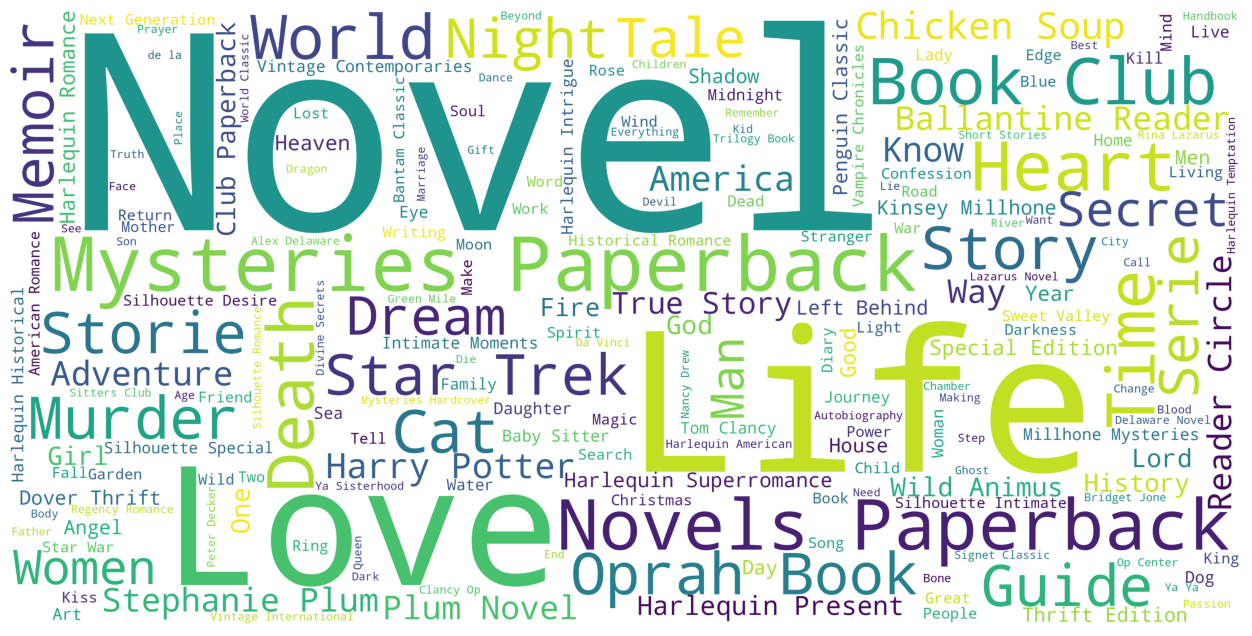
\includegraphics[scale=0.3]{book-title.png}

\begin{itemize}
\item[$\blacksquare$] {\footnotesize Book-Title을 토큰화한 후 WordCloud하였을 때 그림과 같은 결과를 보였습니다. 책 제목에 많이 사용되는 키워드는 Novel, Love, Life 등이 있었으며 Mysteries와 같은 장르나 paperback(soft cover)와 같은 제본 양식 등이 자주 등장했습니다.} 

\end{itemize}
\end{frame}

%---------------------------------------------------------
%---------------------------------------------------------
%Highlighting text
\begin{frame}
\frametitle{EDA}

\centering
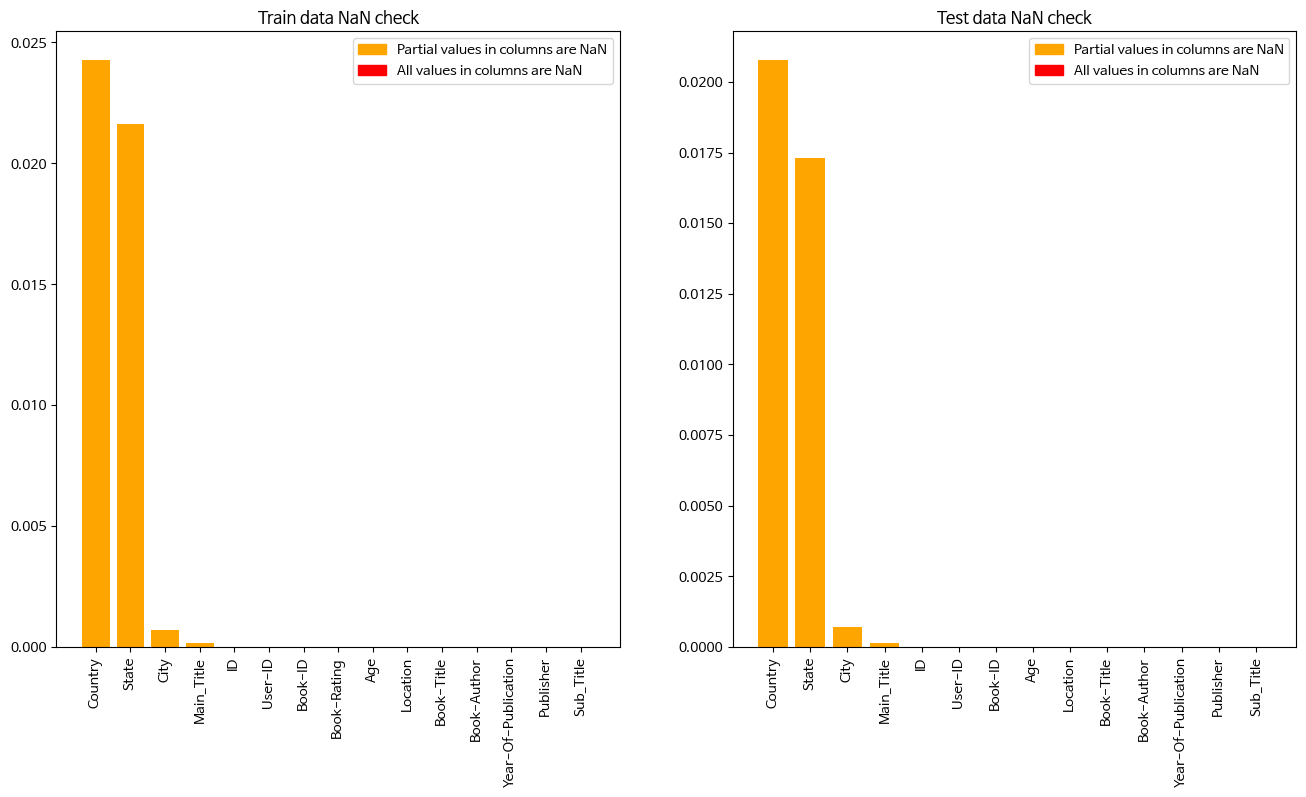
\includegraphics[scale=0.28]{nan_data.png}

\begin{itemize}
\item[$\blacksquare$] {\footnotesize Book-Title과 Location을 re.sub를 통해 특수문자를 제거하고, Title은 Main, Sub로 분할('  '로 구분)하고, Location은 ','를 기준으로 도시, 주, 나라로 나누었을 때 'na'나 ''의 값을 갖는 Null의 빈도는 그림과 같았음.} 

\end{itemize}
\end{frame}

%---------------------------------------------------------

%---------------------------------------------------------
%Highlighting text
\begin{frame}
\frametitle{EDA}

\centering
\begin{minipage}{.5\textwidth}
  \centering
  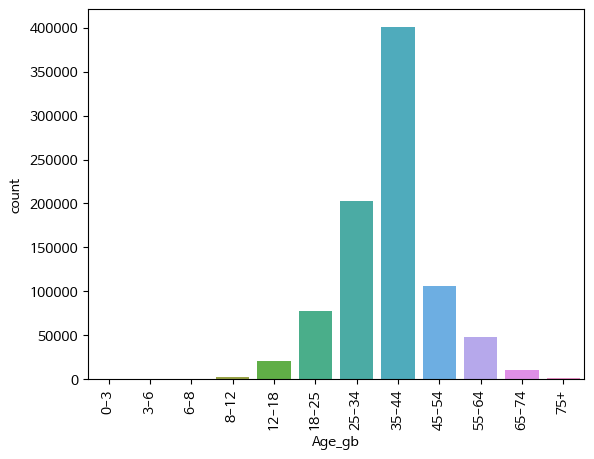
\includegraphics[scale=0.4]{age_gb.png}
\end{minipage}%
\begin{minipage}{.5\textwidth}
  \centering
  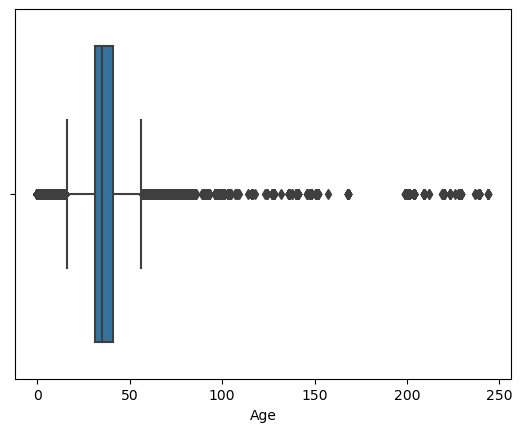
\includegraphics[scale=0.38]{AGE BOXPLOT.png}
\end{minipage}

\begin{itemize}
\item[$\blacksquare$] {\footnotesize 나이대 범주화는 미국 노동통계국에서 발표한 'Spending and employment related to books and other reading materials'를 참고하였습니다. 35-44 사이의 나이대에 리뷰가 제일 많았습니다. 또한 boxplot으로 표현하였을 때, 0세 근방과 100세 이상의 이상치를 확인할 수 있었습니다.} 

\end{itemize}
\end{frame}

%---------------------------------------------------------

%---------------------------------------------------------
%Highlighting text
\begin{frame}
\frametitle{EDA}

\centering
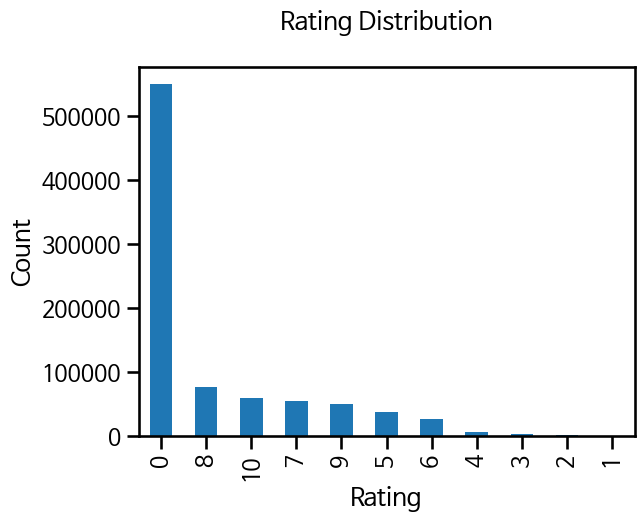
\includegraphics[scale=0.46]{rating distribution.png}

\begin{itemize}
\item[$\blacksquare$] {\footnotesize Train 데이터에서 점수 분포는 그림과 같습니다. 약 87만 개의 데이터 중에 55만개 데이터가 0의 평가입니다. 즉, 유저가 해당 도서에 관심이 없고 관련이 없는 경우가 가장 많았습니다.} 

\end{itemize}
\end{frame}

%---------------------------------------------------------
\subsection{Preprocessing}
%---------------------------------------------------------

%---------------------------------------------------------
%Highlighting text
\begin{frame}
\frametitle{EDA}
\framesubtitle{Preprocessing}

\centering
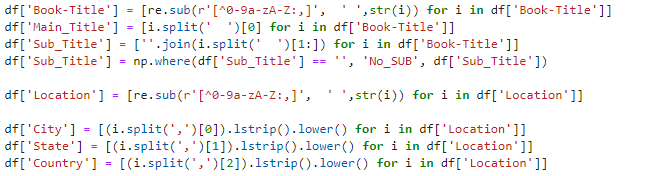
\includegraphics[scale=0.6]{title, location split.png}

\begin{itemize}
\item[$\blacksquare$] {\footnotesize Book-title은 특수문자 제거 후 Main과 Sub Title로 나누었습니다. 이유는 특정 출판사명이나 책 시리즈 등의 부제가 붙기 때문에 나누어 피쳐로 두는 것이 좋다고 생각했습니다. Sub Title이 없는 경우엔 'NO\_SUB'로 바꾸었습니다. Title을 Split한 점이 모델 예측에 좋았습니다.} 

\end{itemize}
\end{frame}
%---------------------------------------------------------

%---------------------------------------------------------
%Highlighting text
\begin{frame}[fragile]
\frametitle{EDA}
\framesubtitle{Preprocessing}

\centering
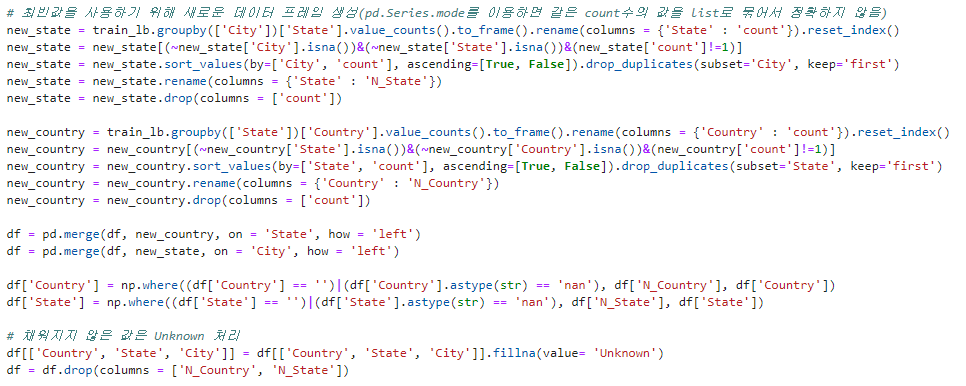
\includegraphics[scale=0.45]{location split.png}

\begin{itemize}
\item[$\blacksquare$] {\footnotesize Location을 도시, 주, 나라로 나눈 뒤 Null은 최빈값으로 대체하였습니다. 처음에는 pandas.Series.mode를 사용하였지만, 해당 agg를 groupby에 적용하면 공통 최빈값은 하나의 list로 묶여져서 value\_counts 후 sort\_values에서 중복 제거 후 첫번째 행을 가져오는 방법을 선택했습니다.} 

\end{itemize}
\end{frame}
%---------------------------------------------------------

%---------------------------------------------------------
%Highlighting text
\begin{frame}
\frametitle{EDA}
\framesubtitle{Preprocessing}

\centering
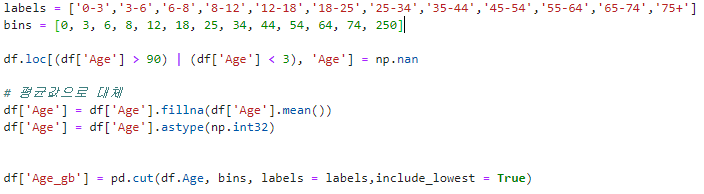
\includegraphics[scale=0.6]{age_gb code.png}

\begin{itemize}
\item[$\blacksquare$] {\footnotesize Age 변수를 나눌 기준을 세우고, 이상치에 해당되는 90세 이상, 3살 미만의 데이터는 Null로 처리한 뒤 평균값으로 대처하였습니다. 기존에 3살 미만은 3살로, 100살 이상은 100살로 고정하는 것보단 좋은 성능을 보였습니다.} 

\end{itemize}
\end{frame}
%---------------------------------------------------------


\section{Model Selection}

%---------------------------------------------------------
%Highlighting text
\begin{frame}[shrink=10]
\frametitle{Model Selection}

{\footnotesize 모델을 선택하기 앞서, 파라미터를 지정하지 않고, random\_state만 고정시킨 뒤, Random forest, Linear Regression, LGB, XGB, Catboost를 돌려서 기본적인 Valid 점수를 확인하고 Catboost를 메인으로 하였습니다. User-ID가 핵심이라 생각해서, 과적합을 방지하기 위해 K-fold 대신 StratifiedKFold를 통해 교차검증하였습니다. }

\begin{center}
$<$History of LB scores$>$
  \begin{tabular}{| c | c | c |}
    \hline
      Model & Describe & Public Score \\ \hline
    Catboost & No\_cat\_features 5-folds & 3.54836                                          \\   \hline
    Catboost & Add\_cat\_features 5-folds& 3.27553                                          \\   \hline
    Catboost & Add\_cat\_features + bertopic 5-folds+optuna& 3.27097                        \\     \hline
    Catboost & Add\_cat\_features 10-folds& 3.26106                                         \\   \hline
    Catboost & stacking(XGB, RF) & 3.40884                                                \\   \hline
    Catboost & Add\_cat\_features 20-folds + preprocessing& 3.26013                         \\   \hline
    Catboost & Add\_cat\_features 20-folds + preprocessing (mean age)& 3.26007                         \\   \hline
    Catboost & Add\_cat\_features 20-folds + preprocessing + title\_split& 3.25811           \\   \hline
  \end{tabular}
\end{center}

\end{frame}
%---------------------------------------------------------
\subsection{Optuna}

%---------------------------------------------------------
%Two columns
\begin{frame}
\frametitle{Model Selection}
\framesubtitle{Optuna}

\begin{columns}

\column{0.5\textwidth}
\textbf{Optuna hyperparameter tuning }\par\medskip
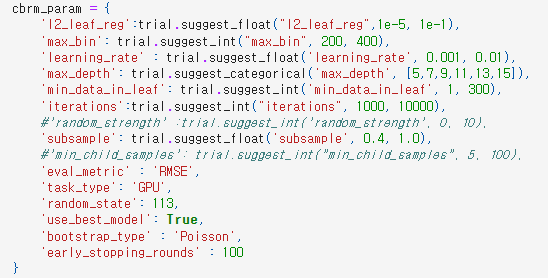
\includegraphics[scale=0.4]{optuna tuning.png}\\

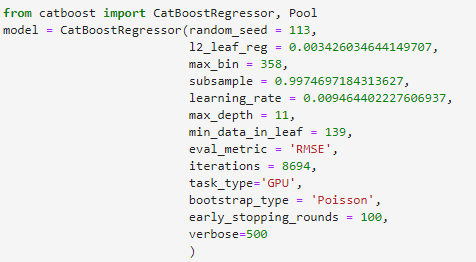
\includegraphics[scale=0.4]{best params.png}\\
\column{0.5\textwidth}
\begin{itemize}
\item[$\blacksquare$] {\scriptsize 대회 metric이 RMSE이고, 점수 복원을 위한 Random state, GPU, 등을 기본적으로 고정하고 중요해보이는 파라미터들만 튜닝하였습니다.}\\
\item[$\blacksquare$] {\scriptsize learning\_rate: 가중치 업데이트 기준}\\
\item[$\blacksquare$] {\scriptsize min\_data\_in\_leaf: leaf의 최소 훈련 샘플 수}\\
\item[$\blacksquare$] {\scriptsize subsample: 각 트리를 훈련하는 데 사용될 features의 비율 (randomly selected)}
\end{itemize}
\end{columns}
\end{frame}
%---------------------------------------------------------

\section{Conclusion}

%---------------------------------------------------------

%---------------------------------------------------------

\subsection{Overall Summary}

%---------------------------------------------------------

%Highlighting text
\begin{frame}
\frametitle{Conclusion}
\framesubtitle{Overall Summary}

\begin{columns}
\column{0.44\textwidth}
\centering

[Final LB Score]\\
\vspace{1.5mm}
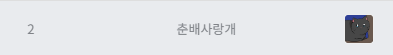
\includegraphics[scale=0.49]{LB rating.png}\\
\vspace{1.5mm}
\begin{tabular}{| c | c |}
  \hline
  LB & Score                    			                \\   \hline
  Public & 3.25811                                          \\   \hline
  Private & 3.27139                                          \\   \hline
\end{tabular}

\column{0.6\textwidth}
\begin{itemize}
\item[$\blacksquare$] {\footnotesize Catboost Regressor를 사용하여 전처리 $+$ 나이 범주화 $+$ 하이퍼파라미터 튜닝 $+$ Ordinal Encoding을 통해 최종 Public 점수는 3.25811, Private 점수는 3.27139를 기록하였습니다.} \\
\item[$\blacksquare$] {\footnotesize 다양한 변수(Title 기반 토픽 모델링, 언어구분, 출판연도 구분, counting 등)를 적용하였지만 기존 변수를 전처리하는 것이 제일 좋은 성능을 보였습니다.}
\end{itemize}
\end{columns}
\end{frame}
%---------------------------------------------------------
%---------------------------------------------------------

%Highlighting text
\begin{frame}
\frametitle{Conclusion}
\framesubtitle{Overall Summary}
\centering
\begin{minipage}{.5\textwidth}
  \centering
  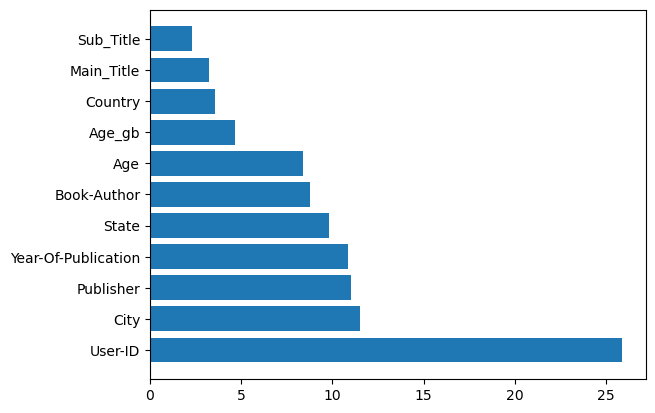
\includegraphics[scale=0.35]{cat_boost importance.png}
\end{minipage}%
\begin{minipage}{.5\textwidth}
  \centering
  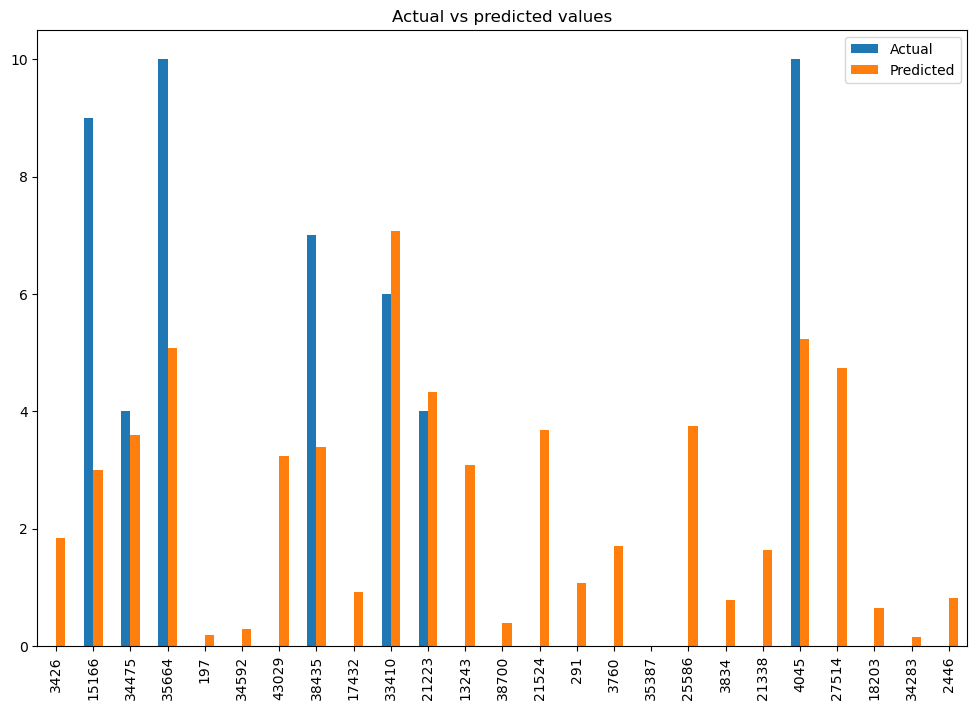
\includegraphics[scale=0.21]{sample pred vs actual.png}
\end{minipage}

\begin{itemize}
\item[$\blacksquare$] {\footnotesize Catboost의 기능 중 feature\_importances\_를 이용하여 트리에서 피쳐가 클래스를 나누는데 얼마나 영향을 미쳤는지 확인할 수 있었습니다. Title은 영향이 상대적으로 적었으며 User-ID가 가장 높고 City, Publisher, Year-Of-Publication이 다음으로 크게 작용했습니다.} 

\item[$\blacksquare$] {\footnotesize Valid set을 얼마나 잘 예측하는지 확인하기 위해서 fold과정에 시각화하는 함수를 넣어 두었습니다. 낮은 점수대는 근사하게 예측하는 반면, 높은 점수대는 잘 예측 못하는 것을 확인할 수 있었습니다.} 
\end{itemize}

\end{frame}
%---------------------------------------------------------

\subsection{Limitation of study}

%---------------------------------------------------------
%Two columns
\begin{frame}
\frametitle{Conclusion}
\framesubtitle{Limitation of study}

\begin{itemize}
\item[$\blacksquare$] {\footnotesize Catboost + 20-folds를 돌렸을 때, 약 4시간 정도 시간이 소모되었는데 fold를 하지않고, 더 많은 것(feature\_importances\_ 관련 feature engineering)을 테스트해봐야 했습니다..}
\item[$\blacksquare$] {\footnotesize Catboost가 아닌 모델들을 Optuna하여 앙상블 모델을 구현했어야 하는데, 시간 관계상 Catboost에만 집중하게 됐습니다.}
\item[$\blacksquare$] {\footnotesize 트리 모델이 아닌 FFM(Field-aware Factorization Machines)도 사용해봤지만 Valid가 3.32까지 나와서 적용하지 못했습니다. 다른 딥러닝 모델도 사용해봐야 했습니다.}
\item[$\blacksquare$] {\footnotesize 점수 분포가 0점에 몰려있어 고 득점대의 예측이 힘들었음. 해당 문제를 해결했다면 RMSE을 조금이라도 줄일 수 있지 않았을까 생각이 들었습니다.}

\end{itemize}

\end{frame}


%---------------------------------------------------------
\begin{frame}
\begin{center}
\Huge Thank You!
\end{center}
\end{frame}
%---------------------------------------------------------
\end{document}